%!TEX root = ../../thesis.tex
\renewcommand{\chapterpath}{\allchapterspath/limitations}
\renewcommand{\imgpath}{\chapterpath/img}

\chapter{Limitations, Extensions and Derivatives}
\label{chapter:limitations}
\minitoc

Context - Why now: We have shown an algortihm that seems to work

Need - Why the reader: we need to know what are the hidden assumption that are really done and how to overcome them. And potential way to go into more complex problems

Task - Why me: I investigated this question and ran some proof of concept experiment that demonstrate my points.

Object - Why this chapter: We list a number of limitation (continuous state, finite set of task, pre-defined unique interaction frame, human is not affected by agent behavior). We then provide ideas to solve that problem and illustrate with some more or less toy example.

Findings - What: We found that there is some limitation and that some direction are shown to be working in simple scenarios.

Conclusions - So what: Let's go work on finding the limitation

Perspectives - What now: 


%%%%%%%%%%%%%%%%%%%%%%%%%%%%%%%%%%%%%%%%%%%%%%
%%%%%%%%%%%%%%%%%%%%%%%%%%%%%%%%%%%%%%%%%%%%%%
%%%%%%%%%%%%%%%%%%%%%%%%%%%%%%%%%%%%%%%%%%%%%%
%%%%%%%%%%%%%%%%%%%%%%%%%%%%%%%%%%%%%%%%%%%%%%
%%%%%%%%%%%%%%%%%%%%%%%%%%%%%%%%%%%%%%%%%%%%%%
\section{Exploiting overlap between distributions}

examplify here the work of AAAI with the bhattacharrya method

%%%%%%%%%%%%%%%%%%%%%%%%%%%%%%%%%%%%%%%%%%%%%%
%%%%%%%%%%%%%%%%%%%%%%%%%%%%%%%%%%%%%%%%%%%%%%
%%%%%%%%%%%%%%%%%%%%%%%%%%%%%%%%%%%%%%%%%%%%%%
%%%%%%%%%%%%%%%%%%%%%%%%%%%%%%%%%%%%%%%%%%%%%%
%%%%%%%%%%%%%%%%%%%%%%%%%%%%%%%%%%%%%%%%%%%%%%
\section{Continuous state space}


In this section we extend our algorithm to a more complex scenario by considering a continuous world, more complex reward functions and the use of both feedback and guidance instructions. We investigate how our algorithm scales to such problem and how different exploration strategies perform.

\subsection{Experimental System}

We now illustrate the application of our algorithm in a more complex problem. This problem is known in the reinforcement learning literature as the \emph{puddle world}. The puddle world consist in a continuous-state MDP in which an agent must reach a goal region while avoiding a penalty region.
% 
In this work we consider a 2 dimensional puddle world with each dimension ranging between 0 and 1. Agent actions are discrete and represent steps in either North, South, East, West direction. One step length is sampled from a normal distribution of mean 0.1 and standard deviation 0.01.

As in the previous experiment, we consider speech as the modality for interacting with the robot and we reuse the dataset used in section~\ref{sec:First}. The interaction scheme is turn taking, where the agent is performing an action and wait for a feedback or guidance signal to continue (see section \ref{sec:mixing}). We only consider a Gaussian classifier.

\subsubsection{Task Representation}
To define the set of possible tasks we project a 5x5 regular grid on top of the continuous world. One task is represented by a +1 reward in one of the 25 projected squares and a -100 reward in three consecutive (vertically or horizontally) squares. +1 and -100 area can not overlap (see figure~\ref{UncertaintyMap}(E) for an example). The set of possible task is defined as all possible combination of such reward function, for a total of 660 hypothesis. 

We use the MDP framework to compute the corresponding policies. The world being continuous we use the tile coding function approximation \cite{sutton1998reinforcement}, with 10 overlapping 50x50 regular grids. %tillins. 
A Q-Learning algorithm \cite{watkins1992q} is used to compute the Q-Values, with a discount rate of 0.99 and a learning rate of 0.01. The hypothesis policies are then defined as greedy according to the Q-Values.

\subsubsection{Exploration strategies}

We will investigate four different agent behaviors. 1) random, 2) $\epsilon$-greedy, 3) myopic uncertainty based exploration, which aim at selecting the action that is the most uncertain in the current state, and 4) full uncertainty based exploration which requires an uncertainty map to decide what to explore next, as presented in Section~\ref{sec:Planning}. 

As we are in a continuous domain we can not compute the full uncertainty for each state as presented in Section \ref{sec:ExplorationMethod}, we therefore approximate this process. Extensions already exist for the continuous state problem \cite{nouri2010dimension,Hester13aamas} and we will rely on a sampling based method. One hundred random states are generated and evaluated in terms of task and instruction uncertainty as described in Algorithm~\ref{alg:u}. Each sampled state is associated to a reward value proportional to its uncertainty which is propagated to neighborhood states by using a fixed Gaussian kernel. We use as amplitude the uncertainty value and a diagonal covariance matrix of value 0.01. The resulting approximated uncertainty map is then used as a reward function in a new MDP problem. By solving this problem, using for instance Q-Learning, the agent plans actions to visit the most uncertain regions. The system can then run an $\epsilon$-greedy policy on this solution. In the following experiment, the agent will use an exploration ratio $\epsilon$ equal to $0.1$.

\subsubsection{Feedback and Guidance Model}
\label{sec:advancedModel}


\subsection{Mixing feedback and guidance}
\label{sec:mixing}

The previously defined teaching signal model limits the use of only feedback or only guidance instruction. Such limitation can be restrictive for the user, we will now consider the case where teachers can use both, i.e. $z \in \{F \cup G\}$. Extending our algorithm to cases where possible meanings include both feedback and guidance requires a probabilistic model of how the teacher distribute feedback and guidance signals. This model must hold the following property $\sum_{i \in \{F \cup G\}} p(z = i|s,a,\hat{\xi})~=~1$. We define a variable $\beta$ that represents the probability of the user providing a feedback signal at each step, i.e. $p(z \in F) = \beta$, which implies $p(z \in G) = 1 - \beta$. 

In \cite{macl11simul} the agent was estimating such protocol parameters from the interaction. In this work we will assume such parameter is known in advance (see Section~\ref{sec:advancedModel}) and further assume it does not depend on the task or on the state of the robot. 
%
Under this new definition we can change the likelihood function to:
%
\begin{eqnarray}
\L_i &=&  p(n_i|s_i,a_i,\hat{\xi},\theta)\nonumber\\
%               &=& \sum_{j} p(n_i|z = j,s_i,a_i,\hat{\xi},\theta)~p(z = j|s_i,a_i,\hat{\xi},\theta)    \nonumber\\
                &=& \sum_{j} p(n_i|z = j,\theta)~p(z = j|s_i,a_i,\hat{\xi}) \nonumber\\
                &=& \sum_{j} p(n_i|z = j,\theta)~w_{ij}^{\hat{\xi}}
                \label{eq:likmix}
\end{eqnarray}
%
with :
%
\begin{eqnarray}
    w_{ij}^{\hat{\xi}} = 
        \begin{cases} 
            \beta~p(z|s_i,a_i,\hat{\xi}) &\mbox{for } z \in F \\
            (1- \beta)~p(z|s_i,\hat{\xi}) & \mbox{for } z \in G
        \end{cases} 
\end{eqnarray}

We consider both feedback and guidance instruction simultaneously. Extending our algorithm to cases where possible meanings include both feedback and guidance requires a probabilistic model of how the teacher distribute feedback and guidance signals. We will use the mixing model described in Section~\ref{sec:mixing} with the individual feedback and guidance model as describe in Section~\ref{sec:fisrtFrame} and a mixing ratio $\beta$ of 0.5. It means that the user is expected to deliver feedback and guidance signals at a similar rate.


\subsection{Results}

We present results from 75 runs of our experiment, where for each run we randomly choose a task to teach from the set of hypothesis as well as the initial state of the agent. For each experiment, we compute the likelihoods every 15 steps and performs a total of 35 updates, for a total of 525 iterations. Figure~\ref{Rmax} shows the average evolution of the taught task hypothesis likelihood.

\begin{figure}[!htbp]
  \centering
  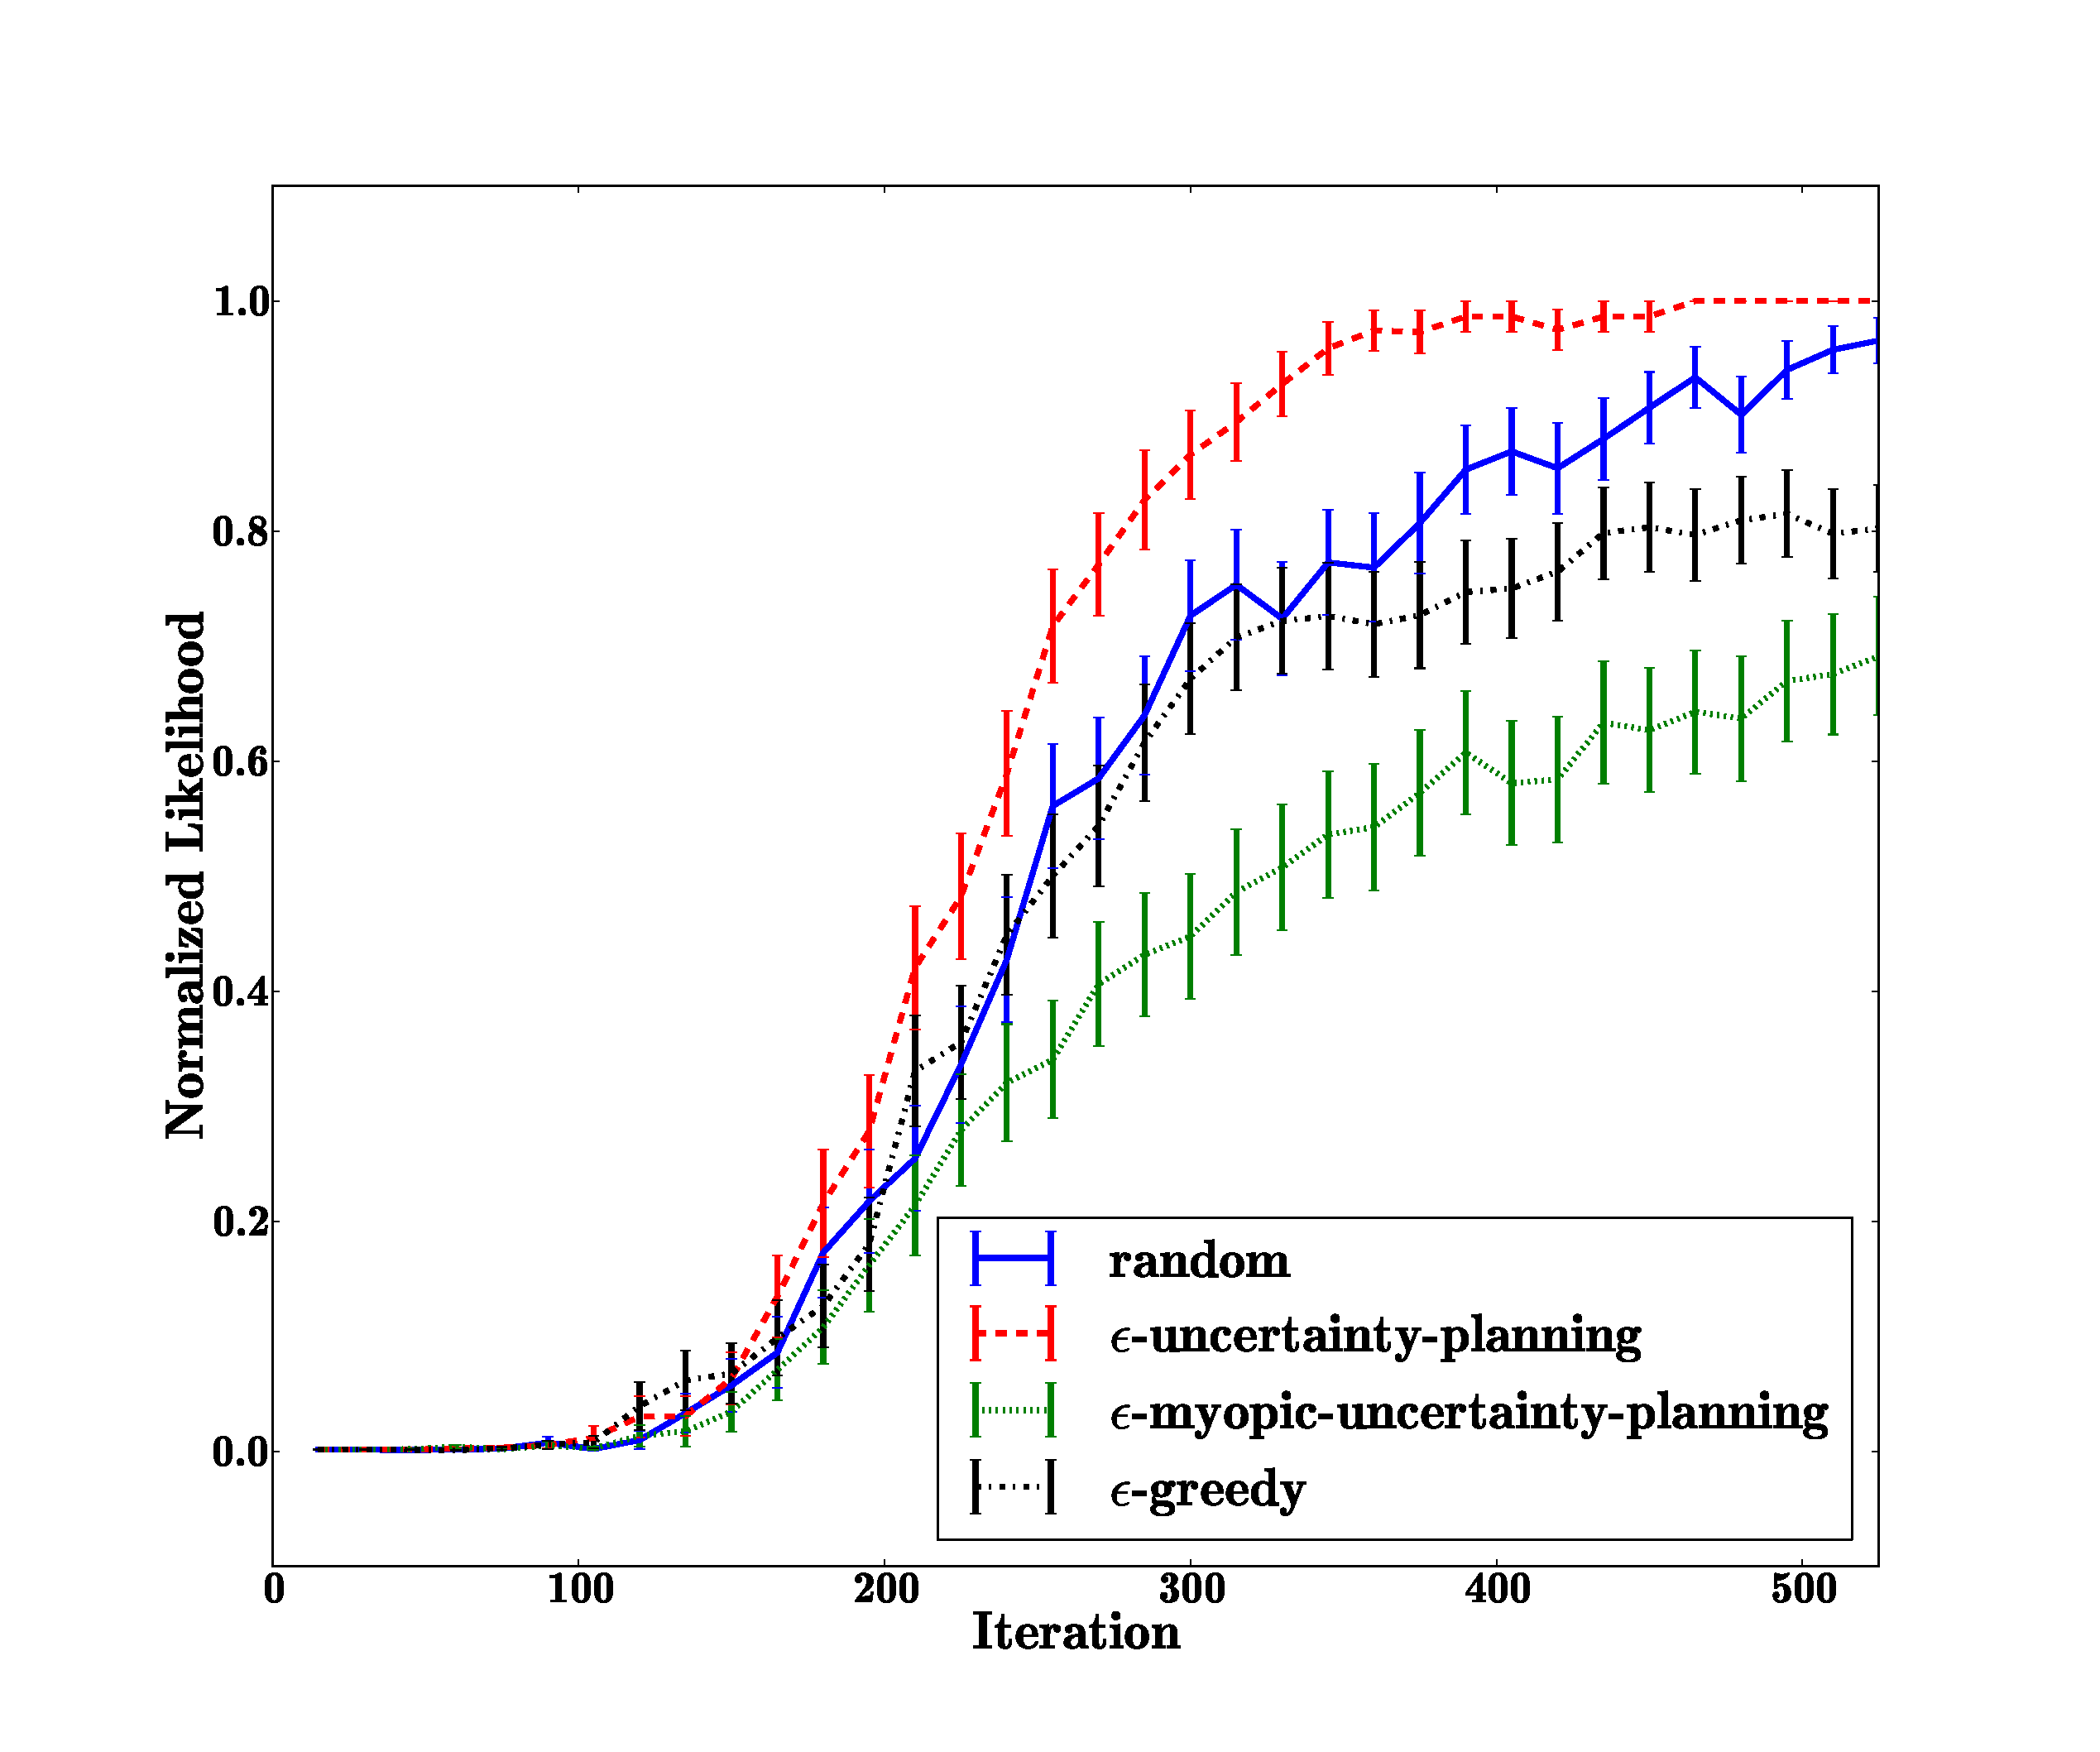
\includegraphics[width=\columnwidth]{\imgpath/continuous}
  \caption{Taught hypothesis normalized likelihood evolution (mean + standard error) thought iteration using Gaussian classifer. Comparaison of different exploration strategies. Uncertainty based exploration method, which plan on the long term, performs significantly better.}
  \label{Rmax}
\end{figure}

Results from figure~\ref{Rmax} show that our algorithm can learn a task in a continuous world from unknown and noisy instructions whose possible meanings are both feedback and guidance and 10\% of the instructions were teaching mistakes. The uncertainty based planning strategy outperforms random action selection. Interestingly, myopic uncertainty based strategy, which is also based on both task and signal uncertainty, is not efficient. This result illustrates some of the issues discussed in section~\ref{sec:Planning}, when considering the agent as not being able to teleport, long term planning is more suited to explore efficiently the state space. 

As expected $\epsilon$-greedy performs less efficiently than in the first setup. This is due to the properties of our new set of hypothesis where many hypothesis shared an identical positive reward area but have different puddle zone.

Figure~\ref{UncertaintyMap} shows the evolution of the estimated uncertainty map for one run of the experiment. For each uncertainty map, the agent plans its actions to reach a maximal uncertainty region. The maximum uncertainty value decreases as the agent is correctly estimating the task.

\begin{figure}[!htbp]
  \centering
      \begin{subfigure}[b]{0.35\columnwidth}
          \centering
          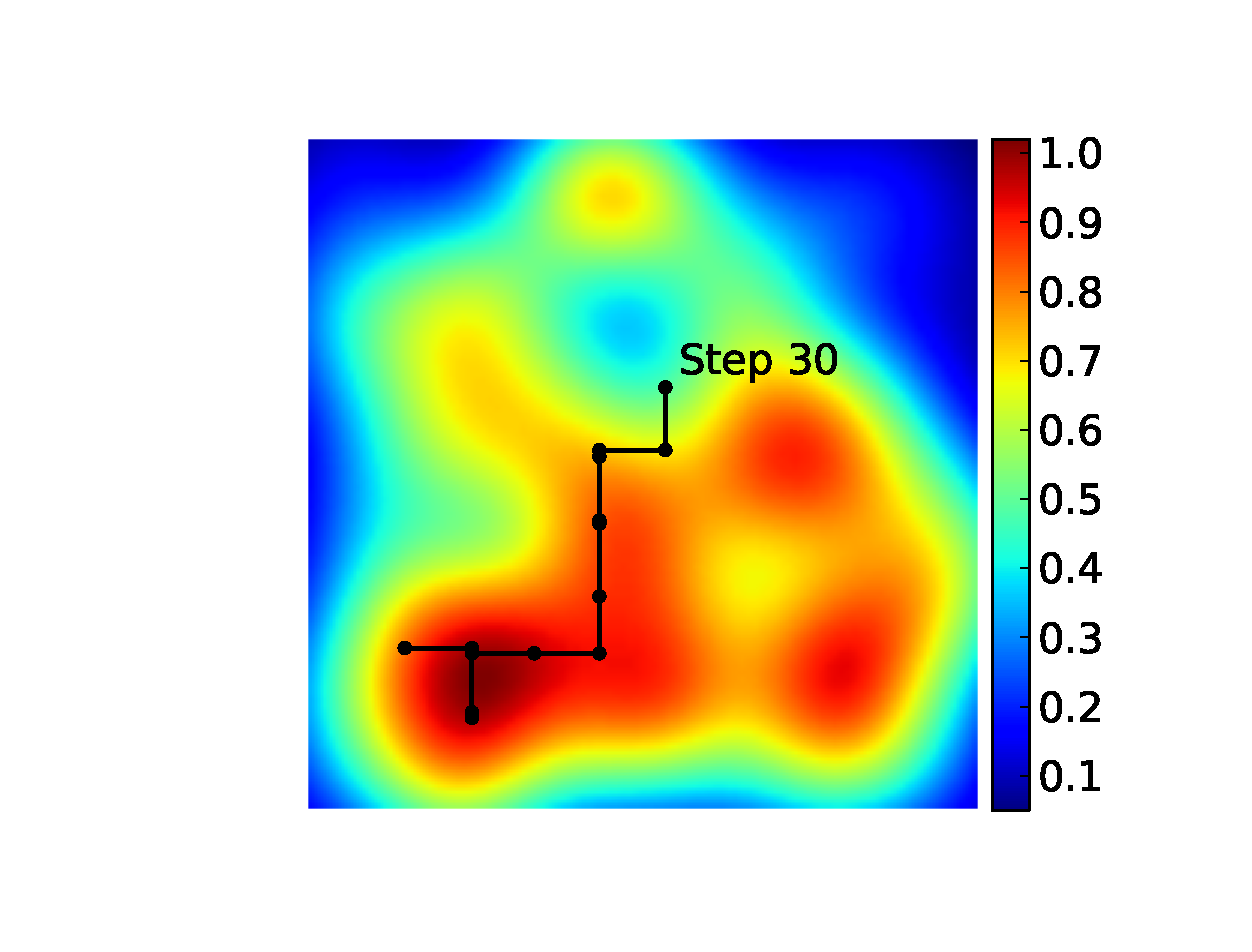
\includegraphics[trim=5cm 1.5cm 1.5cm 1.5cm, clip=true, width=\columnwidth]{\imgpath/30}
          \caption{After 30 iterations.}
          \label{fig:30}
      \end{subfigure}
      \begin{subfigure}[b]{0.35\columnwidth}
          \centering
          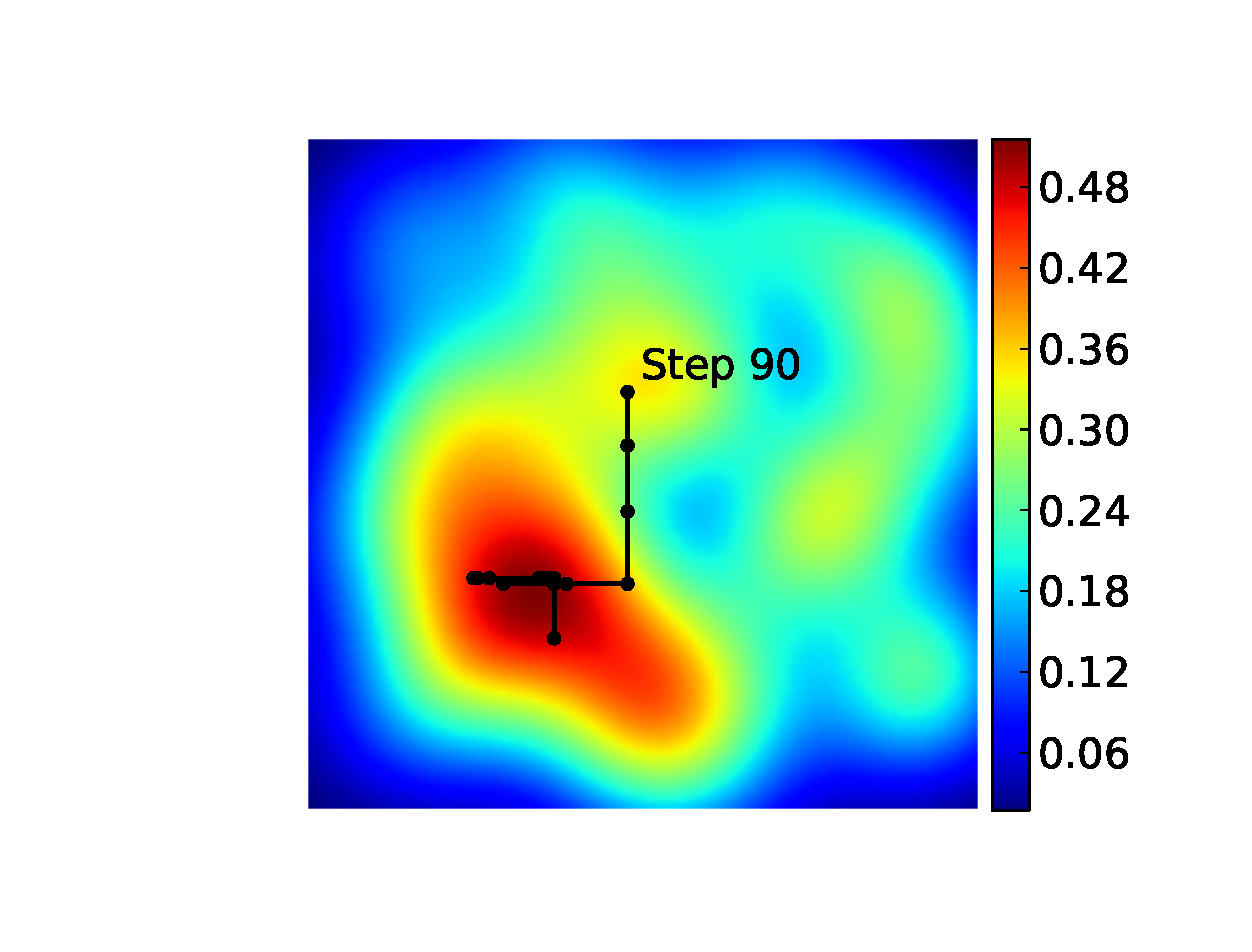
\includegraphics[trim=5cm 1.5cm 1.5cm 1.5cm, clip=true, width=\columnwidth]{\imgpath/90}
          \caption{After 90 iterations.}
          \label{fig:90}
      \end{subfigure}\\
      \begin{subfigure}[b]{0.35\columnwidth}
          \centering
          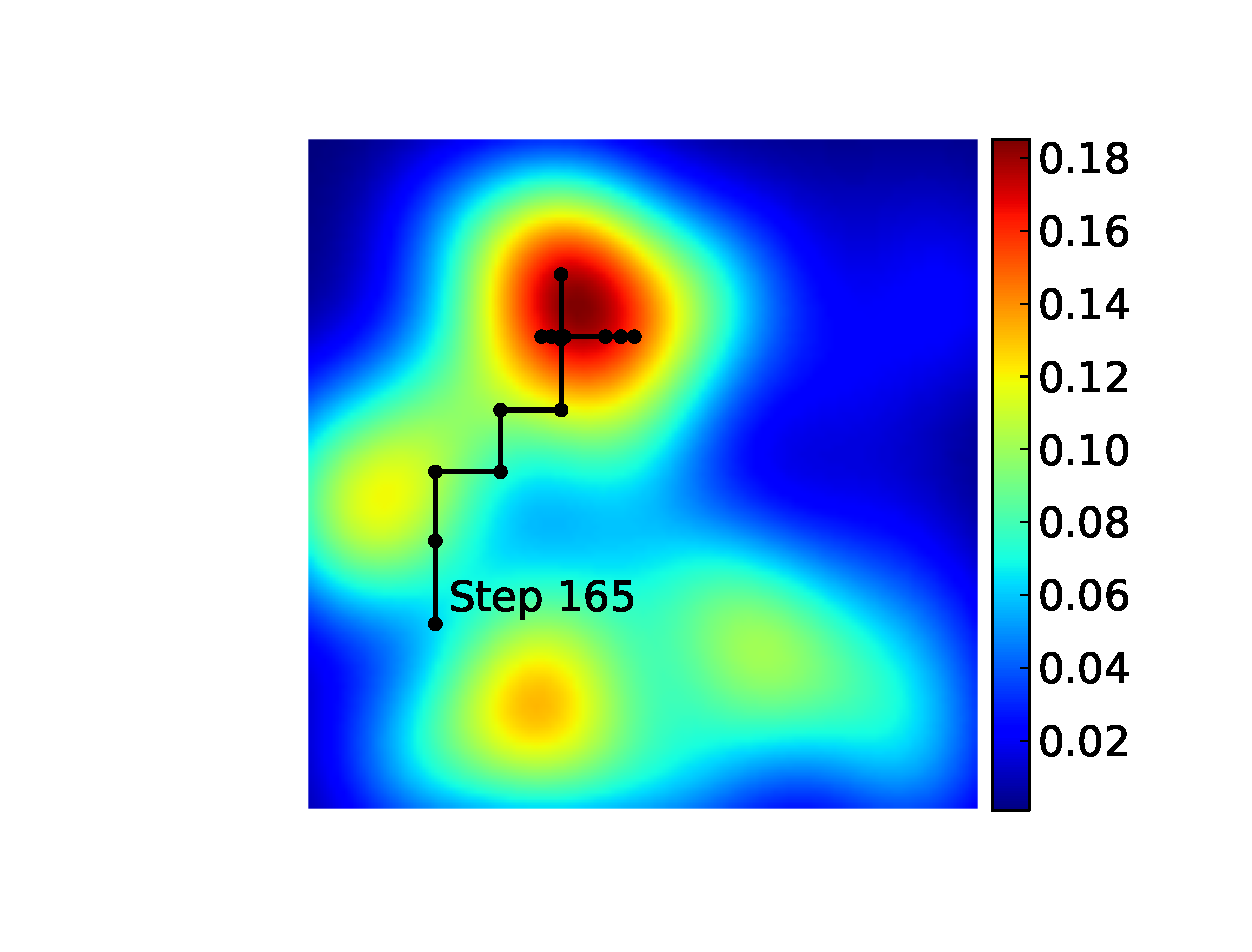
\includegraphics[trim=5cm 1.5cm 1.5cm 1.5cm, clip=true, width=\columnwidth]{\imgpath/160}
          \caption{After 165 iterations.}
          \label{fig:165}
      \end{subfigure}
      \begin{subfigure}[b]{0.35\columnwidth}
          \centering
          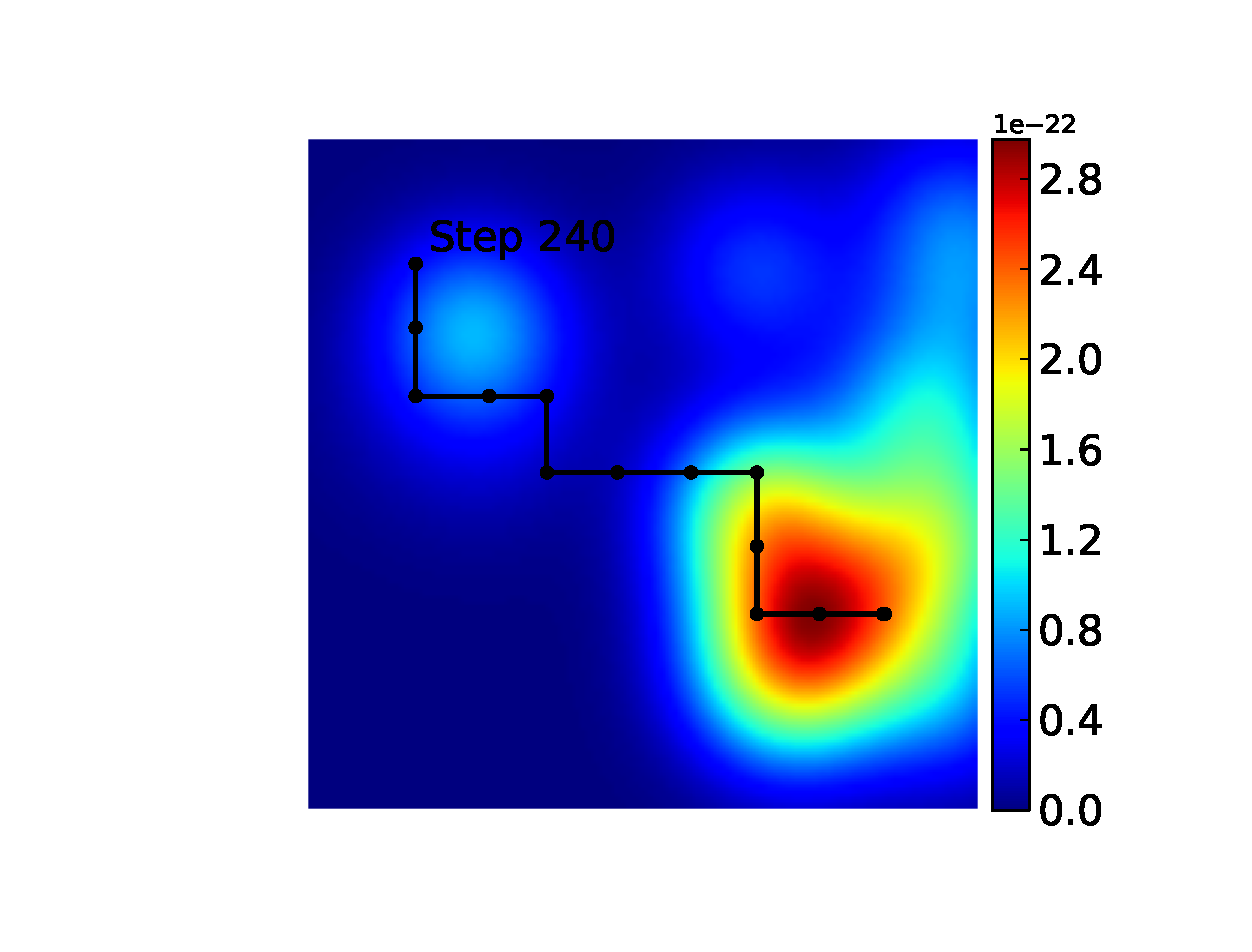
\includegraphics[trim=5cm 1.5cm 1.5cm 1.5cm, clip=true, width=\columnwidth]{\imgpath/240}
          \caption{After 240 iterations.}
          \label{fig:240}
      \end{subfigure}\\
      \begin{subfigure}[b]{0.25\columnwidth}
          \centering
          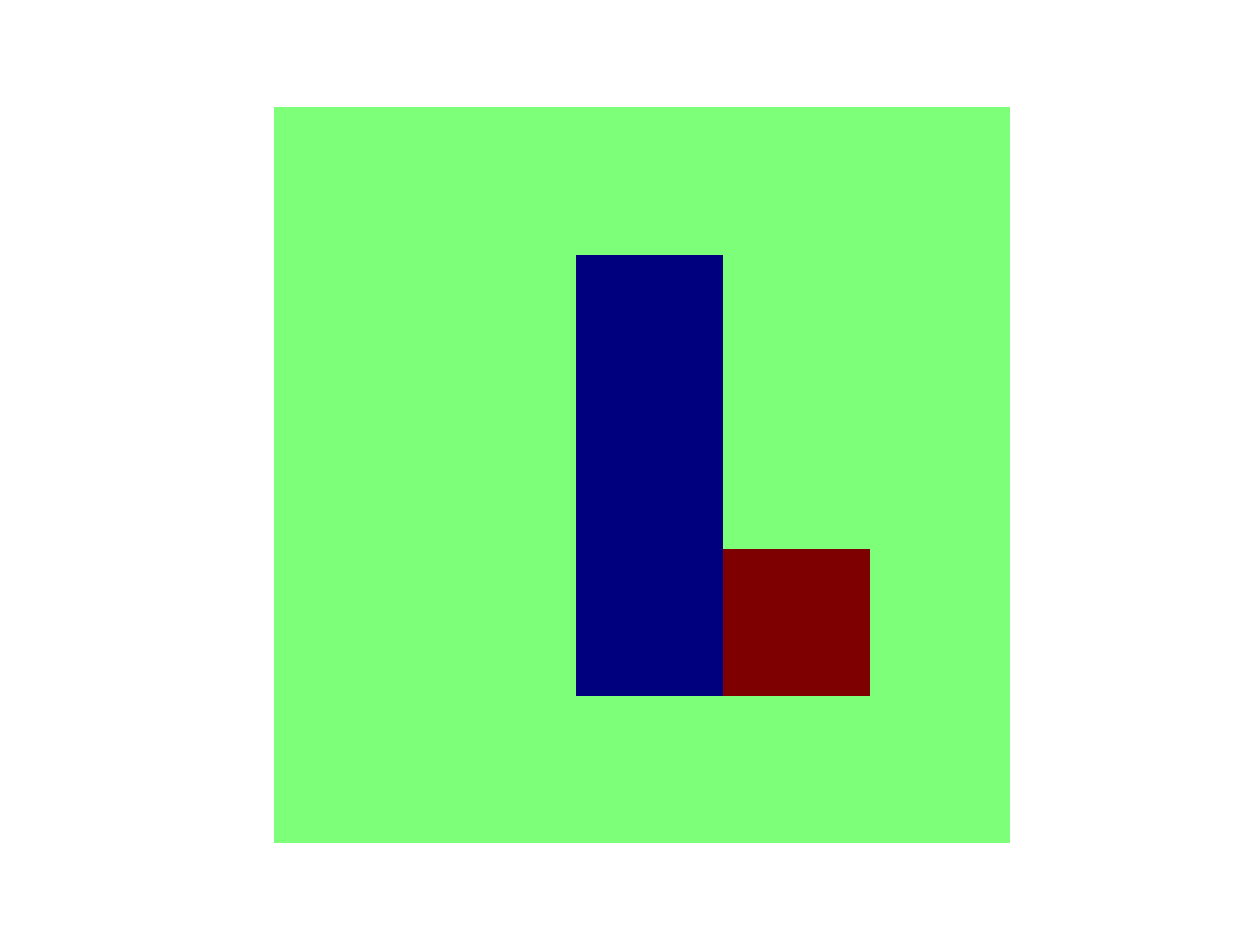
\includegraphics[trim=4cm 1cm 3.5cm 1cm, clip=true, width=\columnwidth]{\imgpath/puddle}     
          \caption{Puddle world used by the teacher.}
          \label{fig:puddle}
      \end{subfigure}
      \begin{subfigure}[t]{0.45\columnwidth}
          \centering
          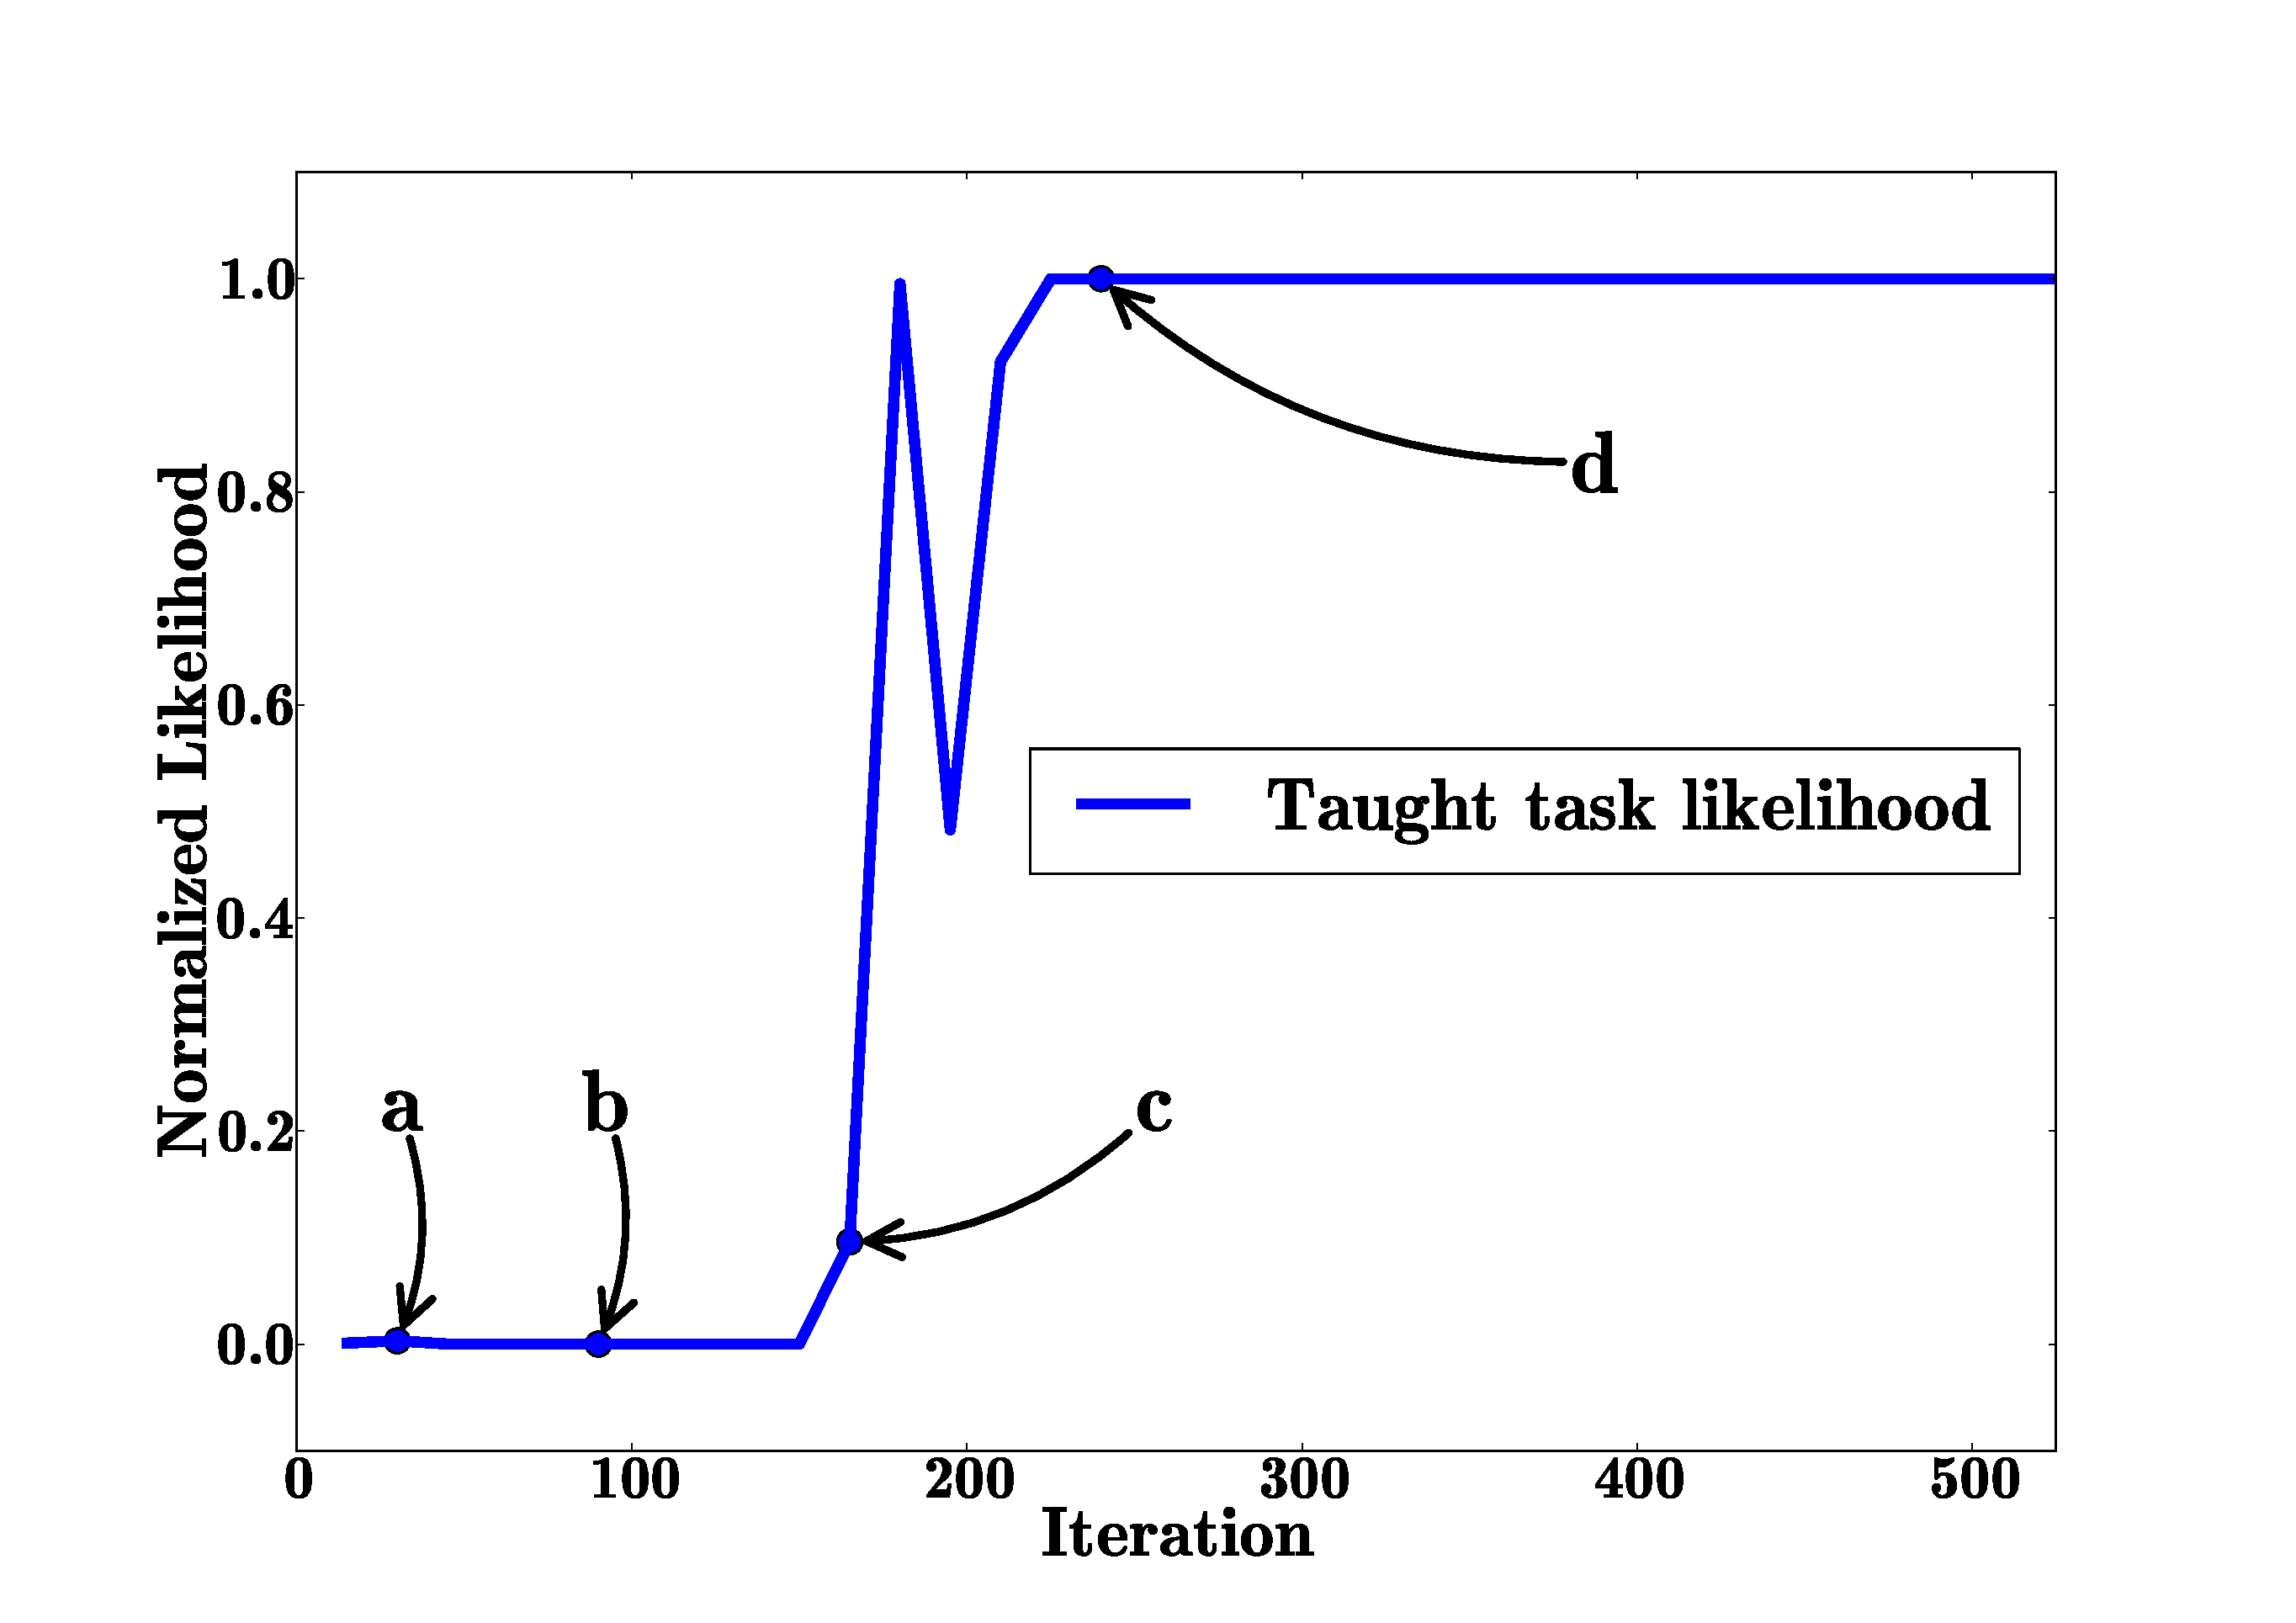
\includegraphics[trim=2cm 1cm 3cm 2cm, clip=true, width=\columnwidth]{\imgpath/evo}
          \caption{Taught hypothesis normalized likelihood evolution.}
          \label{fig:evo}
      \end{subfigure}
        
  \caption{Log Uncertainty maps after a) 30, b) 90, c) 165 and d) 240 iterations. e) shows the puddle world choosen by the teacher and f) shows the learning progress and the frame associated to each of the uncertainty map. In order to display the differences between log values, we bounded the colormap between -5 and 0, which correspond to uncertainty values between 0.0067 and 1. Some log values, especially for d), are lower than -5 and are displayed in the same color as -5. Best shown in color.}
  \label{UncertaintyMap}
\end{figure}

%%%%%%%%%%%%%%%%%%%%%%%%%%%%%%%%%%%%%%%%%%%%%%
%%%%%%%%%%%%%%%%%%%%%%%%%%%%%%%%%%%%%%%%%%%%%%
%%%%%%%%%%%%%%%%%%%%%%%%%%%%%%%%%%%%%%%%%%%%%%
%%%%%%%%%%%%%%%%%%%%%%%%%%%%%%%%%%%%%%%%%%%%%%
%%%%%%%%%%%%%%%%%%%%%%%%%%%%%%%%%%%%%%%%%%%%%%
\section{Continous set of hypothesis}
\label{chapter:limitations:continoushypothesis}

a simple particle filter

How to leverage from the finite set of hypothesis constraint? A potential avenue is to use a combination of particle filter and regularization on the task space.

\paragraph{Pre-defined finite set of tasks and instruction meanings} In order to make the learning problem tractable, it was assumed in this article that the robot learner knows that the task to be learnt can be approximated by one task among a pre-defined set of tasks. Indeed, without constraining the space of possible tasks, an infinite number of reward functions may explain the particular teaching data received by the robot. In practice, the number of pre-defined tasks in the experiment was still relatively large (624), allowing a certain level of flexibility. Yet, it would be highly desirable to extend the possibility to deal with continuous task representation, allowing potentially infinite spaces of tasks. A potential avenue to address this would be to constrain search through a combination of regularization and particle filter approaches. The space of tasks to be sampled at a given moment may also be constrained by the current situation and context (for example, a robot hearing the instructions of a human while he is looking at cubes on a table may infer that the task has a higher probability to be defined in terms of manipulation of these cubes than to change the state of an object in another room). Similarly, the system assumed a pre-defined repertoire of possible meanings to be associated with continuous instruction signals. Extending the system towards the creation of novel meanings is an important question. Another approach, for both extending task and meaning repertoires dynamically, would be to allow the user to teach the robot new macro-actions, associated to new macro-instructions, or macro-state, for example based on the options framework \cite{sutton1999between}.

%%%%%%%%%%%%%%%%%%%%%%%%%%%%%%%%%%%%%%%%%%%%%%
%%%%%%%%%%%%%%%%%%%%%%%%%%%%%%%%%%%%%%%%%%%%%%
%%%%%%%%%%%%%%%%%%%%%%%%%%%%%%%%%%%%%%%%%%%%%%
%%%%%%%%%%%%%%%%%%%%%%%%%%%%%%%%%%%%%%%%%%%%%%
%%%%%%%%%%%%%%%%%%%%%%%%%%%%%%%%%%%%%%%%%%%%%%
\section{Pre-defined interaction frame}
first freeze the number of task and find the correct interaction frame from a set of interaction frame
second, have two set, one for the frame one for the task

%%%%%%%%%%%%%%%%%%%%%%%%%%%%%%%%%%%%%%%%%%%%%%
%%%%%%%%%%%%%%%%%%%%%%%%%%%%%%%%%%%%%%%%%%%%%%
%%%%%%%%%%%%%%%%%%%%%%%%%%%%%%%%%%%%%%%%%%%%%%
%%%%%%%%%%%%%%%%%%%%%%%%%%%%%%%%%%%%%%%%%%%%%%
%%%%%%%%%%%%%%%%%%%%%%%%%%%%%%%%%%%%%%%%%%%%%%
\section{Human in the loop}

In real-world applications, users are usually told how to interact with machines. Do people want to have an open-ended choice about what signal to use? Would they be more efficient? When is it better to use a calibration procedure?

how does the agent behavior affect the algorithm assumption on human behavior

Assumption: The properties of the signals do not change wrt. the behavior of the agent

Users comply with the frame implemented. Same meaning, optimal strategies, timing...

discuss how the setup can be used in HRI, but also semiotic stuff...

\paragraph{Usability and user studies}

Only prerecorded datasets have been used. However, signals may change during the learning. For instance, people can try to adapt themselves to a robot if they believe the latter is not understanding properly. Or, brain signals are sensitive to the protocol, the duration of the experiment or even the percentage of errors made by the agent \cite{chavarriaga2010learning}. To which extend the behavior of our agent changes the properties of the teaching signal? Can we adapt to such changes online? 

As we argued in the introduction, the work we presented is a starting point towards forms of adaptive interaction with non-technical users, that we may call fluid interaction learning. While we studied in this article properties of learning algorithms that will be needed for such an endeavor, it remains to be shown how they can be integrated within a full real-world human-robot interaction scenario and architecture so that the usability and acceptability of such system can be evaluated. Thus, user studies in particular will be a crucial next step of this work. Some improvements of the system may be needed to reach acceptable levels of usability.
Indeed, our current system can be restrictive for the user as the number of interaction increases quickly with the complexity of the size of the task and meaning spaces. However, we have shown that the system is able to use known sources of information, which in real-world interaction could be leveraged to keep the sample complexity low.

In relation to targeting fluid interaction learning, we will consider in the future how more complex kinds of instructions can be included in our formalism. Indeed, the possible teaching models used spontaneously by people can be more complex than the simple meaning correspondences we assumed \cite{thomaz2008teachable,Cakmak2010optimality}. Also the turn taking scheme could be made more natural, as the robot could ask questions \cite{cakmak2012designing} and accept asynchronous instructions.

%%%%%%%%%%%%%%%%%%%%%%%%%%%%%%%%%%%%%%%%%%%%%%
%%%%%%%%%%%%%%%%%%%%%%%%%%%%%%%%%%%%%%%%%%%%%%
%%%%%%%%%%%%%%%%%%%%%%%%%%%%%%%%%%%%%%%%%%%%%%
%%%%%%%%%%%%%%%%%%%%%%%%%%%%%%%%%%%%%%%%%%%%%%
%%%%%%%%%%%%%%%%%%%%%%%%%%%%%%%%%%%%%%%%%%%%%%
\section{Word properties}
xp with a grid world versus a real maze with many wall and see that random becomes a joke

\paragraph{Symmetric task repertoires} Our approach assumes that the robot is equipped with planning skills and can not be used if several hypothesis are fully symmetric as they will not be differentiable. This latter problem can be solved by redefining the set of hypothesis, for instance by adding a ``stop'' action valid only at the goal states.

How the task properties (symmetries, size, \ldots) affect the learning properties?

%%%%%%%%%%%%%%%%%%%%%%%%%%%%%%%%%%%%%%%%%%%%%%
%%%%%%%%%%%%%%%%%%%%%%%%%%%%%%%%%%%%%%%%%%%%%%
%%%%%%%%%%%%%%%%%%%%%%%%%%%%%%%%%%%%%%%%%%%%%%
%%%%%%%%%%%%%%%%%%%%%%%%%%%%%%%%%%%%%%%%%%%%%%
%%%%%%%%%%%%%%%%%%%%%%%%%%%%%%%%%%%%%%%%%%%%%%
\section{No need for MDP}


%%%%%%%%%%%%%%%%%%%%%%%%%%%%%%%%%%%%%%%%%%%%%%
%%%%%%%%%%%%%%%%%%%%%%%%%%%%%%%%%%%%%%%%%%%%%%
%%%%%%%%%%%%%%%%%%%%%%%%%%%%%%%%%%%%%%%%%%%%%%
%%%%%%%%%%%%%%%%%%%%%%%%%%%%%%%%%%%%%%%%%%%%%%
%%%%%%%%%%%%%%%%%%%%%%%%%%%%%%%%%%%%%%%%%%%%%%
\section{Coherent means nothing}


%%%%%%%%%%%%%%%%%%%%%%%%%%%%%%%%%%%%%%%%%%%%%%
%%%%%%%%%%%%%%%%%%%%%%%%%%%%%%%%%%%%%%%%%%%%%%
%%%%%%%%%%%%%%%%%%%%%%%%%%%%%%%%%%%%%%%%%%%%%%
%%%%%%%%%%%%%%%%%%%%%%%%%%%%%%%%%%%%%%%%%%%%%%
%%%%%%%%%%%%%%%%%%%%%%%%%%%%%%%%%%%%%%%%%%%%%%
\section{A minimalist proof}

lack of proof

\subsection{Interpretation hypothesis: a symbolic signal example}

We further assume that the user is coherent and uses one signal for one meaning. The assumption is that the mapping between symbolic signals and their meaning can only be of two forms.

It could be exemplified by an interface with two buttons, one for ``correct'' and one for ``incorrect'', but the mapping between the button and the meaning would not be defined in advance.

\todo{figure with possible mapping}

For a particular hypothesis, the robot can assign hypothetic meanings)to the human signals knowing their are limited to a fixed set and according to the current state of the world. The machine is ``reasoning'' as follow: \emph{"If the human wants me to solve task G1 then when I performed action $a$ in state $a$ and he said ``oui'', he meant ``incorrect''"}. 

\todo{example step by step, first the world, one action, it interpretation wrt. each hypothesis, then accelerate and observe}

By creating a set of hypothesis, the system end-up with a set of possible interpretation of the human teaching signals. But as the user have only one objective in mind, here G1, only the correct interpretation will exhibit a coherence between the signals and their associated meanings. 

In our case, as the user is using symbolic signals, and that we assumed the user is coherent and use always the same symbol for the same meaning. We can infer that hypothesis G1 is the correct one as the resulting mapping between signal and meaning is more coherent.

\todo{For the symbolic case, and given specific constraint we will present a minimalist proof once the associated mathematical notation will be introduced}

The example described above simplifies the problem in some aspects. Indeed we assume the robot is already able to discriminate between perceptual events and has access to a unlabeled symbolic representation of the teaching signals. It would be the case when using a button based interface, however, when considering more ``natural'' means of interaction such as speech, the mapping between spoken words and their meaning should be learn by the machine. Indeed, the same word in never pronounced exactly the same way and some classification algorithm should be applied to train a discriminative model.




